\documentclass{emulateapj}
\submitted{{\it Submitted for publication in ApJL}}
\usepackage{multirow,color,wrapfig,ulem}
\usepackage {graphicx}

\usepackage{amsmath} 
\usepackage{amssymb} 
\usepackage{graphics}
\usepackage{epsfig}  
\usepackage{float}
\bibliographystyle{apj}
\def\be{\begin{equation}}
\def\ee{\end{equation}}
\def\ba{\begin{eqnarray}}
\def\ea{\end{eqnarray}}

\newcommand{\avg}[1]{\langle{#1}\rangle}  
\newcommand{\hMpc}{{\ifmmode{h^{-1}{\rm Mpc}}\else{$h^{-1}$Mpc }\fi}}  
\newcommand{\hGpc}{{\ifmmode{h^{-1}{\rm Gpc}}\else{$h^{-1}$Gpc }\fi}}  
\newcommand{\hmpc}{{\ifmmode{h^{-1}{\rm Mpc}}\else{$h^{-1}$Mpc }\fi}}  
\newcommand{\hkpc}{{\ifmmode{h^{-1}{\rm kpc}}\else{$h^{-1}$kpc }\fi}}  
\newcommand{\hMsun}{{\ifmmode{h^{-1}{\rm {M_{\odot}}}}\else{$h^{-1}{\rm{M_{\odot}}}$}\fi}}  
\newcommand{\hmsun}{{\ifmmode{h^{-1}{\rm {M_{\odot}}}}\else{$h^{-1}{\rm{M_{\odot}}}$}\fi}}  
\newcommand{\Msun}{{\ifmmode{{\rm {M_{\odot}}}}\else{${\rm{M_{\odot}}}$}\fi}}  
\newcommand{\msun}{{\ifmmode{{\rm {M_{\odot}}}}\else{${\rm{M_{\odot}}}$}\fi}}  
\newcommand{\bullb}{MACS J0025.4-1222}
\newcommand{\bulla}{1E0657---56} 
\shorttitle{Bullet Groups}
\shortauthors{Fern\'andez-Trincado et al.}

\begin{document} 

\title{Bullet Groups as a test of $\Lambda$CDM}
\author{J. G. Fern\'andez-Trincado$^{1,2,3}$, J. E. Forero-Romero$^1$
  and T. Verdugo$^3$} 
\affil{$^1$ Departamento de F\'{i}sica, Universidad de los Andes,
  Cra. 1 No. 18A-10, Edificio Ip, Bogot\'a, Colombia\\ 
       $^2$ Institute Utinam, CNRS UMR6213, Universit\'e de
  Franche-Comt\'e, OSU THETA de Franche-Comt\'e-Bourgogne,
  Besan\c{c}on, France\\ 
       $^3$ Centro de Investigaciones de Astronom\'ia, AP 264,
  M\'erida 5101-A, Venezuela}        

\begin{abstract}
We estimate the expected distribution of displacements between the two
dominand dark matter peaks in halos within a mass range corresponding
to galaxy groups. We find that the probability of finding a system
similar with displacements of $\sim$400 kpch$^{-1}$ is between 40\%
for z$=0$ and 60\% for z$=1$ and $\Lambda$CDM standard model, which
correspond to the observational constraint the object SL2S J08544-0121
that is  a gravitational lens found in the SL2S and located at
z$=0.35$. Given the larger abundance of groups with respect to
clusters, finding multi-modal groups and baryonic-dark matter
displacements.  
\end{abstract}

\begin{keywords}
{cosmology: theory -- dark matter} 
\end{keywords}

\section{Introduction}


This paper is organized as the follows. In Section
\ref{sec:simulation} we present the simulation and the halo catalogs
used in this work. We continue in Section \ref{sec:setup} with the
geometry of the problem at hand and the measurements setup. Next in
Section \ref{sec:results} we present our results to finish with a
discussion and conclusion in Sections \ref{sec:discussion} and
\ref{sec:conclusions}. 


\section{Simulation and halo catalogs}
\label{sec:simulation}

The analysis presented in this paper uses mainly the Bolshoi (250
Mpch$^{-1}$ simulation box, 1 kpch$^{-1}$ resolution) Database
simulation described in \citet{2011ApJ...740..102K}. The simulation
follows the evolution of 8.6 billion particle cosmological N-body
simulation from z=80 to z=0 in a comoving cube of $250$ Mpch$^{-1}$
on a side. The cosmology used  corresponds to  the spatially flat
concordance model with the following parameters:  the density
parameter for matter (dark matter$+$baryons) $\Omega_m=0.27$, the
density parameter for baryonic matter  $\Omega_b=0.0469$, the density
parameter for dark energy $\Omega_{\Lambda}=0.73$, the Hubble
parameter $h=0.7$, the 
normalization of the Power spectrum $n=0.95$ and the amplitude of mass
density fluctuation (at redshift z$=$0) $\sigma_8=0.82$.  The number
of particles used for each of the DM component was $2048^3$, resulting
in a mass resolution of $1.35 \times 10^8$ M$_{\odot}$h$^{-1}$.   

\section{Bullet Geometry and Measurement Setup}
\label{sec:setup}


\section{Results}
\label{sec:results}

\subsection{Cumulative Probability Distributions}
\label{cumulative_distribution}

We selected four snapshot of the simulation for four different
redshifts (z$=0$, z$=0.25$, z$=0.5$ and z$=1$) based in the
distribution of redshift in the Figure 1 by \citet{verdugo}, and  for
each sample in redshift we selected the host halo with circular
velocities greater than 300 kms$^{-1}$ and was split in two  principal
groups: The first group correspond to host halo with circular
velocities between 300 kms$^{-1}$ to 700 kms${^{-1}}$ with mass in the
range of $10^{12}$ M$_\odot{}$ to $10^{14}$ M$_\odot{}$ in the range
of mass of the Bullet Groups, and second group correspond to host halo
with circular velocities greater than 700 kms$^{-1}$ with mass
$\geq10^{14}$ M$_\odot{}$, in the range of mass of the Bullet
Clusters, in  the Table \ref{table1} is shown the two groups selected
in this work. For each group, we  classified the corresponding
substructures most massive and associated with the corresponding host
halo. The configuration of this system is shown in  Figure
\ref{configuration}, where you  an distinguish the host halo and
substructure for a particular configuration in z$=0$. In  this work,
we estimate the expected distribution of displacements
($d_{real,(X,Y)}$) in the projection 2-D that can estimate by
observations, these displacements correspond to the separation between
the minimal potential of the host halo and the  minimal potential of
the substructure, both are dark matter distributions. 


\begin{table*}
\begin{center}
\begin{tabular}{ccccccc}\hline\hline
Sample       & Minimum Mass           & Maximum Mass          & \# Halos  & \# Halos  & \# Halos & \# Halos \\
             & M$_{\odot}$h$^{-1}$    & M$_{\odot}$h$^{-1}$   &   $z=0$   & $z=0.25$  & $z=0.5$  & $z=1$  \\\hline
Host Halo    & 0.35$\times{}10^{14}$  & 1.09$\times{}10^{14}$ &    400    &   362     &   310    &  192   \\
Substructure & 0.38$\times{}10^{11}$  & 0.30$\times{}10^{14}$ &    400    &   362     &   310    &  192   \\\hline
\end{tabular} 
\caption{Mass ranges for the two groups selected in this work in different redshifts.}
\label{table1}
\end{center}
\end{table*}


In order to explore the distribution of displacements expected in the observational, we define a new parameter given by:\\

\begin{equation}
 \frac{\nu_{circ,sub}}{\nu_{circ,halo}}=0.5
\end{equation}
 

Figure \ref{newparameter} shows the scatter plot of the parameter $\left(\frac{\nu_{circ,sub}}{\nu_{circ,halo}}\right)$ vs the 
displacement ($d_{2d,(X,Y)}$) between the host halo and the substructure and for different redshifts. This parameter is 
consistent with the observations. The red star simbol in the Figure \ref{newparameter} is equal to 0.54 corresponding to 
the fraction in velocity dispersion in the line-of-sigth of the group SL2S SJ08544-0121 ($\sigma_{host,halo}=341^{+43}_{-109}$ kms$^{-1}$ and $\sigma_{substructure}=185^{+30}_{-62}$), reported by \citet{2013A&A...552A..80M}.
Based in the parameter $\left(\frac{\nu_{circ,sub}}{\nu_{circ,halo}}\right)>0.5$, we estimate the expected distribution of
displacements and this is shown in the Figure \ref{displacements} for the two groups classified in this work.
 
  
\begin{figure*}
\begin{center}
%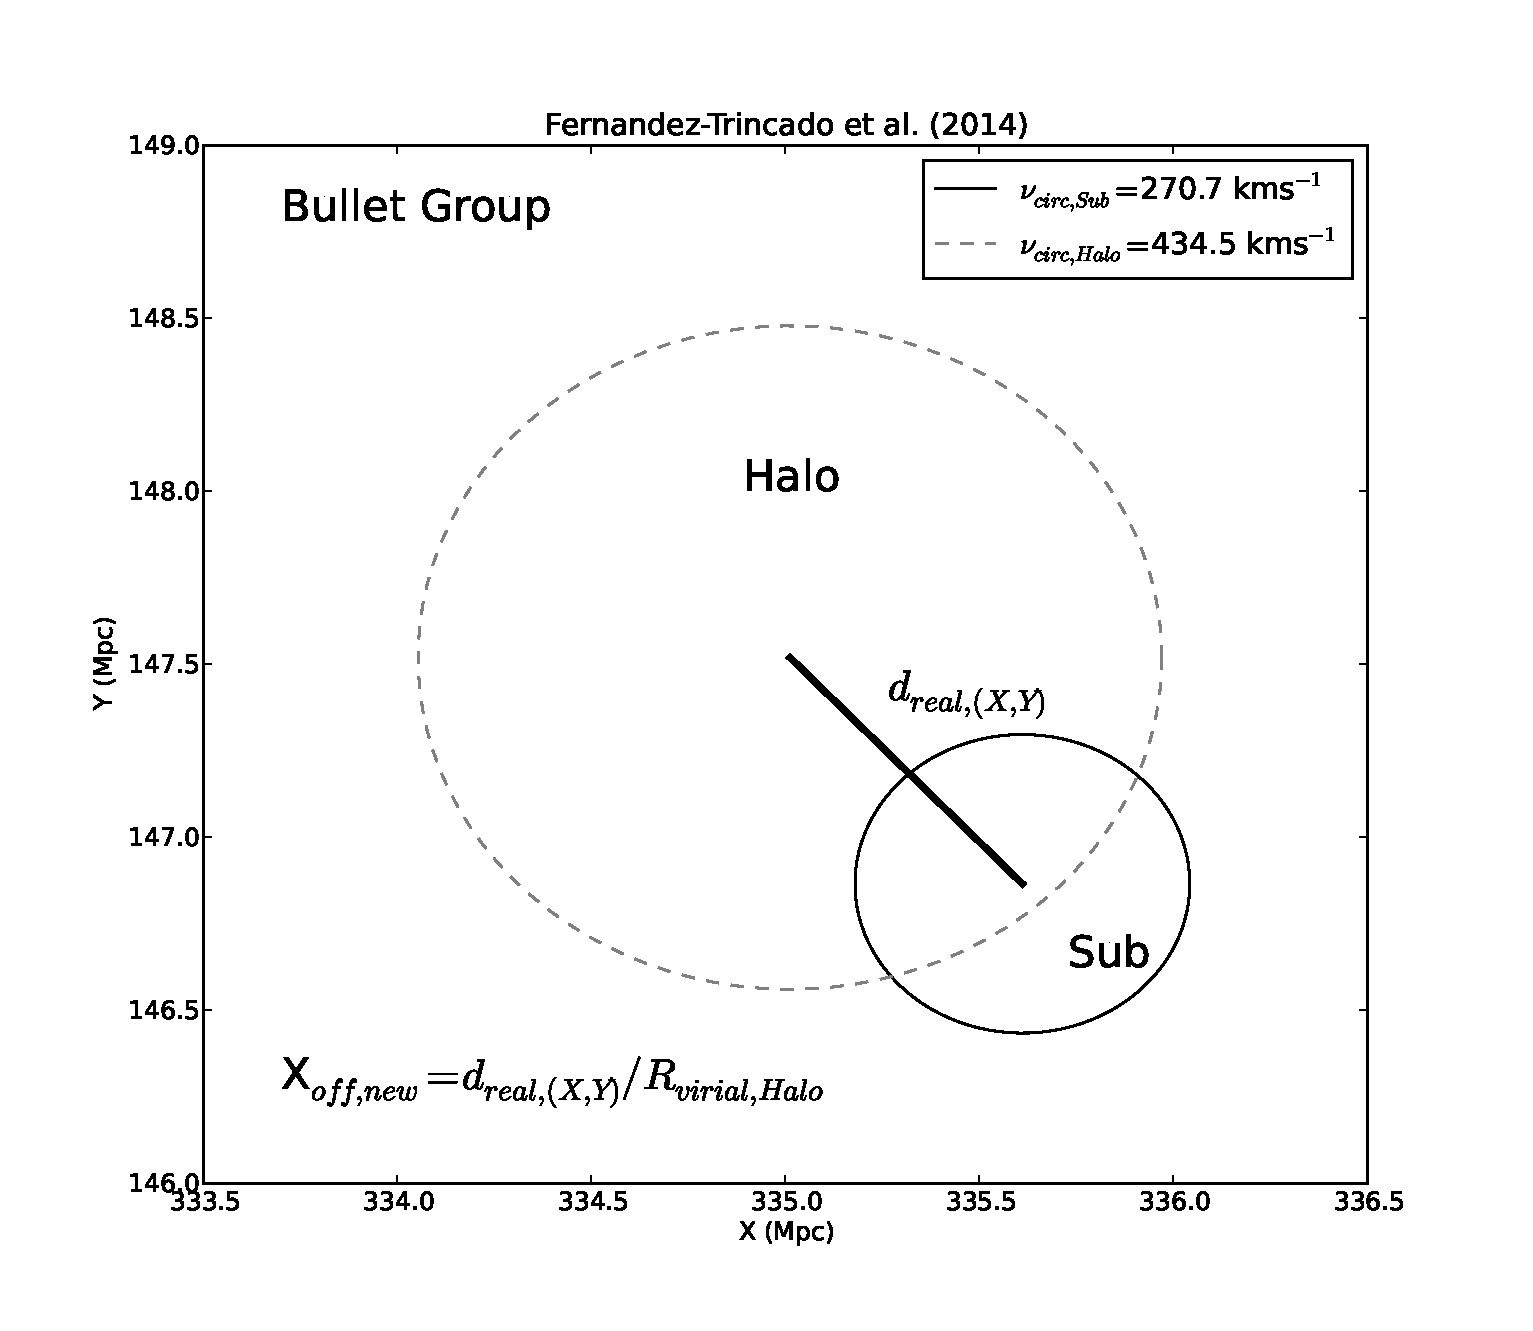
\includegraphics[width=0.90\textwidth]{Bullet_Group.eps}
\end{center}
\caption{Configuration for a host halo (dashed circle) and sub-structure (black circle) in the sample. } 
\label{configuration}
\end{figure*}


\begin{figure*}
\begin{center}
%\includegraphics[width=1.0\textwidth]{Figures_eps/figure_7_2.eps}
%\includegraphics[width=1.0\textwidth]{Figures_eps/figure_7_3.eps}
\end{center}
\caption{Scatter $\left(\frac{\nu_{circ,sub}}{\nu_{circ,halo}}\right)$
  vs $d_{2d,(X,Y)}$ for different redshifts. The  horizontal dashed
  line correpond to
  $\left(\frac{\nu_{circ,sub}}{\nu_{circ,halo}}\right)=0.5$ and the
  red star simbol correspond to
  $\left(\frac{\nu_{circ,sub}}{\nu_{circ,halo}}\right)=0.54$ for SL2S
  SJ08544-0121 in \citet{2013A&A...552A..80M}. The  four top panels
  are the sample with circular velocities $>700$ kms$^{-1}$ and the
  four down panels are the sample with  circular velocities between
  300 km s$^{-1}$ to 700 kms$^{-1}$.} 
\label{newparameter}
\end{figure*}



\begin{figure*}
\begin{center}
\includegraphics[width=1.1\textwidth]{Figures_eps/figure_7_1.eps}
\end{center}
\caption{Cumulative distribution (P$>d_{2d,(X,Y)}$) of displacements
  for the projection (X,Y). {\bf Left panel:} Sample with
  $\nu_{max}>700$ kms$^{-1}$  for different redshifts. The vertical
  dashed line, correspond to the separation between dark matter to
  dark matter estimate in this work as the double of separation
  between the collisional gas and dark matter of 124$\pm$20 kpc
  reported by \citet{gastaldello} for the group SL2S J08544-0121.
  {\bf Right panel:} Sample with $300 $ kms$^{-1} <\nu_{max}<700 $
  kms$^{-1}$ for different redshifts.}  
\label{displacements}
\end{figure*}


\subsection{Number expected of Bullet Groups in the sample}


In order of estimate the number of Bullet Groups expected in the Bolshoi Cosmological Simulation, we 
define the configuration of this system as one where the substructure is coming out of the host halo ($cos(\theta)>0.5$). For this 
we make the scalar product between the velocity vector and position vector that defines the separation between 
 the host halo and the substructure, as shown below: \\
 
 \begin{equation}
  cos(\theta)=\frac{\vec{\nu{}}\cdotp{}\vec{r}}{\left\|\nu{}\right\| \left\|r\right\|}
 \end{equation}

where, $\vec{\nu{}}=\vec{\nu}_{sub}-\vec{\nu}_{halo}$ and $\vec{r}=\vec{r}_{sub}-\vec{r}_{halo}$, in the Figure \ref{cos_theta}
is shown the scatter plot of $cos(\theta{})$ vs $X_{off,new}=\frac{d_{2d,(X,Y)}}{R_{virial,halo}}=\frac{d_{real,(X,Y)}}{R_{virial,halo}}$.  


\begin{figure*}
\begin{center}
%\includegraphics[width=1.0\textwidth]{Figures_eps/figure_8_1_nu=0.5_300kms_700kms.eps}
\end{center}
\caption{Scatter of $cos(\theta)$ vs $X_{off,new}$. The red dashed line correpond to the limit for $cos(\theta{})>0.5$,  
where the substructure is emerging from the host halo and  $\left(\frac{\nu_{circ,sub}}{\nu_{circ,halo}}\right)\geq0.5$, 
cicular velocities $<700$ kms$^{-1}$ and different redshifts.} 
\label{cos_theta}
\end{figure*}

\begin{figure*}
\begin{center}
%\includegraphics[width=1.0\textwidth]{Figures_eps/figure_8_3_nu=0.5_300kms_700kms.eps}
\end{center}
\caption{Cumulative distribution of $d_{real, (X,Y)}$ for $cos(\theta)>0.5$, $\left(\frac{\nu_{circ,sub}}{\nu_{circ,halo}}\right)\geq0.5$, 
cicular velocities $<700$ kms$^{-1}$ and different redshifts.} 
\label{cumulative_cos}
\end{figure*}


\section{Discussion}
\label{sec:discussion}



\section{Conclusions}
\label{sec:conclusions}


\section*{Acknowledgements}

The CosmoSim database used in this paper is a service by the
Leibniz-Institute for Astrophysics Potsdam (AIP). The  BolshoiP
simulation was performed within the Bolshoi project of the University
of California High-Performance  AstroComputing Center (UC-HIPACC) and
was run at the NASA Ames Research Center. 


\bibliographystyle{apj}
\bibliography{references} 

\end{document}
